\chapter{The Targeted Proteolysis module}
\label{chap:enzdig}

The module Targeted Proteolysis is designed to post-process the mass spectrometry data acquired during the enzymatic proteolysis of a target protein by a single protease. In a typical experimental setup both the protease and the target protein are mixed together under various experimental conditions and the peptides generated during the proteolysis are identified by mass spectrometry. It is expected that several control experiments and several replicates of the tested experimental conditions are performed. The main objective of the module is to identify the peptides with intensity values that are significantly different in the control experiments and the replicates of the various experimental condition tested at the chosen significance level. 

\section{Definitions}

Before explaining in detail the interface and how does the module works, lets make clear the meaning of the term Filtered peptide in the context of the Targeted proteolysis module:

\phantomsection
\begin{itemize}
	\item \textit{Filtered peptide}: a relevant peptide with a significantly different behavior in the control and a given experiment at the chosen significance level.\label{par:PIP}
\end{itemize}

\section{The input data files}

The Targeted Proteolysis module requires a data file containing the detected peptides and a sequence file containing the amino acid sequence of the recombinant protein used in the study. Both files must follow the guidelines specified in \autoref{sec:datafile}. In short, the data file must have a tabular format with tab separated columns and the name of the columns are expected as first row. The sequence file is expected to contain only one sequence and to be FASTA formatted with or without the header line. All columns given as input in the section \textit{Column numbers} in Region \num{2} of the interface must be present in the data file. Optionally, another sequence file with the sequence of the native target protein and a pdb file may be specified.

\section{The interface}

The window of the Targeted Proteolysis module is divided in four regions (\autoref{fig:enzdigmw}). 

Region \num{1} contains four buttons allowing users to quickly delete all provided input and start a new analysis. The Clear all button will delete all user provided input and will empty the list box in Region \num{3}. The Clear files button will delete the path to all user provided files and will empty the list box in Region \num{3}. The Clear values button will delete all user provided input for the section Values in Region \num{2}. Finally, the Clear columns button will delete all user provided column numbers. 

Region \num{2} contains the fields where users provide the information needed in order to perform the post-processing of the input data file. The section \textit{Files} in Region \num{2} will provide the path to the input data and output files. It contains six buttons. 

\num{1}.- The Data file button allows users to browse the file system and select a data file. Only .txt files can be selected here. Once the data file is selected, the name of the columns in the file will be shown in the list box in Region \num{3}. If the path to the data file is typed in, the display of the name of the columns in Region \num{3} can be trigger by pressing the Enter key in the keyboard while the Data file entry box has the focus of the keyboard.

\num{2}.- The Sequence (rec) button allows users to browse the file system and select the file containing the sequence of the recombinant protein under study. Only .txt or .fasta files can be selected here. Alternatively,  a UNIPROT code may be given in this field.

\num{3}.- The Sequence (nat) button allows to select the file containing the sequence of the native protein. Only .txt or .fasta files can be selected here. Alternatively, a UNIPROT code may be given in this field. The sequence of the native protein is an optional field. A value of NA means that no native sequence file will be given. 

\num{4}.- The PDB file button allows to browse the file system to select a .pdb file. The .pdb file should contain the structure of the Target protein. This .pdb file will be used to map the cleavages detected in the MS experiments to the structure of the protein. This is an optional field. A value of NA means that no .pdb file will be given. See page \pageref{par:pdbID} for more details. 

See \autoref{sec:datafile} for more details about the data files.

\begin{figure}[h]
	\centering
	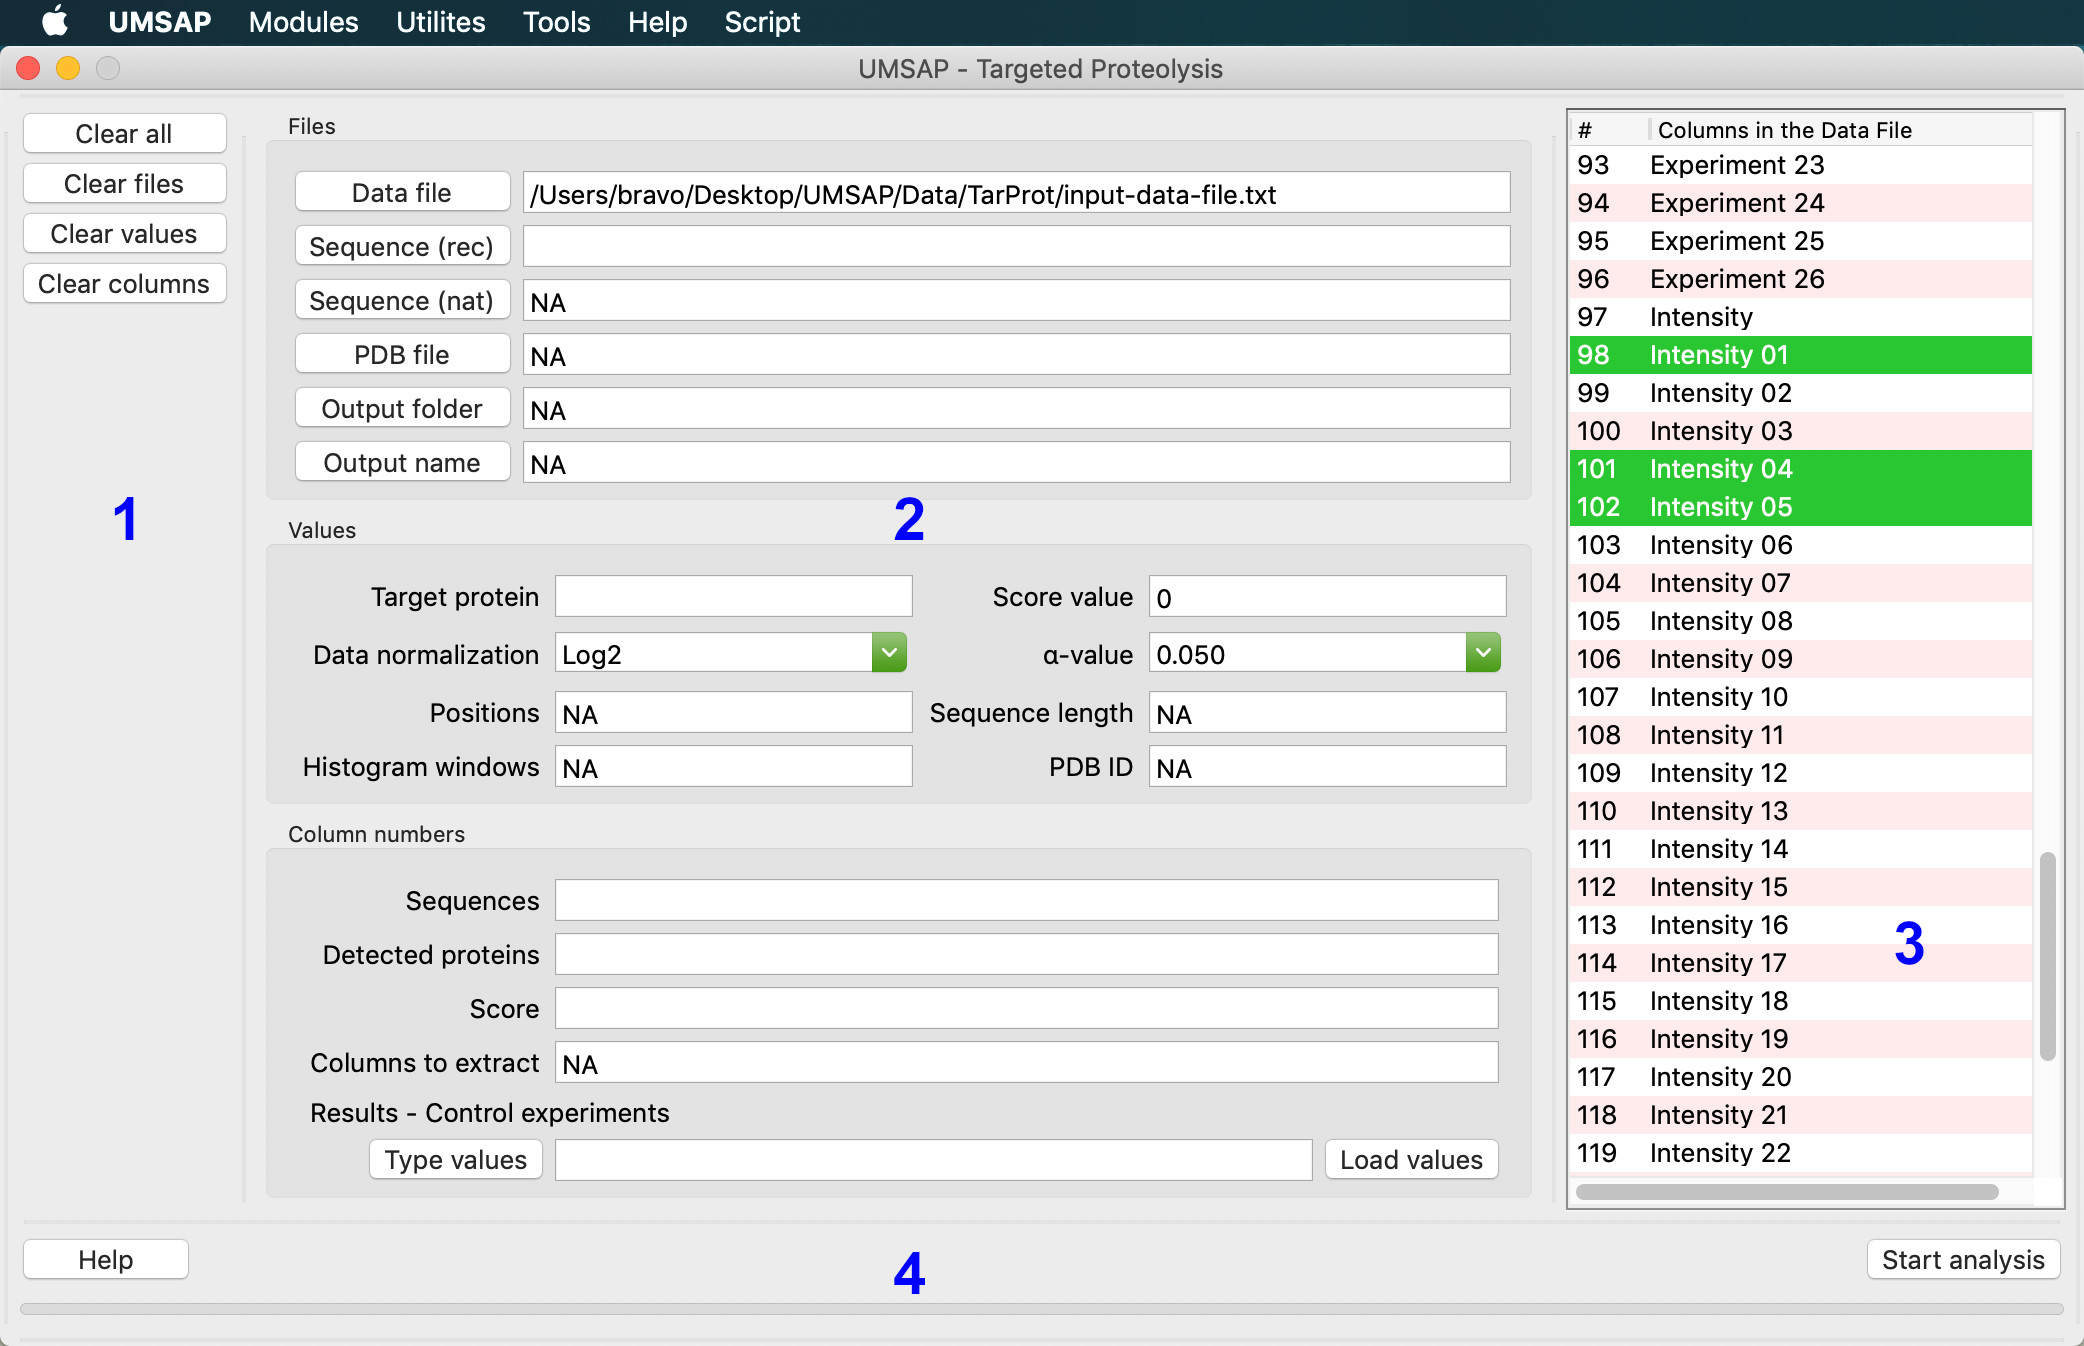
\includegraphics[width=0.7\textwidth]{./IMAGES/MOD-TARPROT/tarprot-mod.jpg}
	\caption[The Targeted Proteolysis window]{\textbf{The Targeted Proteolysis window.} This window allows users to performed the analysis of the results obtained during an enzymatic proteolysis experiment. Optional parameters default to NA when the window is created. The rest of the parameters must be provided by the user.} 
	\label{fig:enzdigmw}
	\vspace{-5pt} 	
\end{figure} 

\phantomsection
\num{5}.- The Output folder\label{par:enzdigOutF} button allows users to browse the file system and select the location of the folder that will contain the output. By default, UMSAP will create a TarProt folder inside the selected Output folder to save all the generated results. If only the name of the output folder is given, the output folder will be created in the same folder containing the data file. If this field is left empty, then the TarProt folder will be created in the same folder containing the data file. If the selected output folder already contains a TarProt folder, then the current date and time to the seconds will be added to the name in order to avoid overwriting the files from previous analyses.

\num{6}.- The Output name button does nothing but the text box to its right allows users to specify the name of the files that will be generated during the analysis. If this field is left empty, then the name tarprot will be used for the output files. 

The section \textit{Values} in Region \num{2} contains eight parameters. Here, users provide information about the target protein, how the data file should be processed and which optional analysis will be performed.

\phantomsection
\num{1}.- The parameter Target protein\label{par:subsprot} allows users to specify which of the proteins detected in the MS experiments was used as substrate during the enzymatic proteolysis. Users may type here any unique protein identifier present in the data file. The search for the target protein is case sensitive, meaning that eFeB is not the same as efeb.

\phantomsection
\num{2}.- The parameter Score value\label{par:scorevalueenzdig} allows users to define a threshold value above which the detected peptides will be considered as relevant. The Score value is an indicator of how reliable was the detection of the peptide during the MS experiments. The value given to UMSAP depends on the program generating the data file. Only one real number equal or greater than zero will be accepted as a valid input here. A value of zero means all detected peptides belonging to the target protein will be treated as relevant sequences.

\num{3}.- The parameter Data normalization allows selecting the normalization procedure to be performed before running the analysis of the data in the data file. Currently, only a $\log_2$ normalization is possible but this will be expanded soon to include quantile, variance stabilization and local regression normalization, among other methods. 

\num{4}.- The parameter $\alpha$-value sets the significance level for the ANCOVA test used to identify peptides with a behavior in the experiments significantly different to the control. See page \pageref{par:ancovatest} for more details.

\phantomsection
\num{5}.- The parameter Positions\label{par:enzdigPos} allows users to define the number of positions to be considered during the amino acid (AA) distribution calculation, see \autoref{subsec:aadistcalc} for more details. Only one integer number greater than zero will be accepted here. A value of NA means that the AA distribution calculation will not be performed. 

\phantomsection
\num{6}.- The parameter Sequence length\label{par:enzdigSeqL} allows users to define the number of residues per line in the short version of the sequence alignment files, see \autoref{subsec:seqali} for more details. Only one integer number greater than zero will be accepted here. A value of NA means that the sequence alignment files will not be generated.

\phantomsection
\num{7}.- The parameter Histogram windows\label{par:enzdigHist} allows users to define the size of the windows for the Histogram analysis, see \autoref{subsec:histocut} for more details. Only integer numbers equal or greater than zero will be accepted here. In addition, the values must be organized from smaller to bigger values. Users may specify a fix histogram window size by given just one integer number greater than zero. In this case the histogram will have even spaced windows with the width specified by Histogram windows. If more than one number is provided here, then windows with the customs width will be created. For example, the input \numlist{50 100} will create only one window including cleavage sites between residues \numrange{50}{99}. The input \numlist{1 50 100 150} will create three windows including cleavages sites between residues \numrange{1}{49}, \numrange{50}{99} and \numrange{100}{149}. Duplicate values are not allowed. A value of NA means that no histograms will be created.

\phantomsection
\num{8}.- The parameter PDB ID\label{par:pdbID} allows users to specify the chain or segment in the pdb file to use when mapping the cleavages detected in the MS experiments to the structure of the target protein. There are two possibilities. When a PDB file is provided with the button PDB file in the section \textit{Files} in Region \num{2} of the interface, then the expected value for PDB ID is only the chain or segment ID found in the pdb file that will be used for mapping the detected cleavages. When the pdb file should be downloaded from the PDB database, then a PDB code and the chain or segment ID is expected here. The format in this case is Code:Chain or Code:SegmentID, for example, 2y4f:A or 2y4f:PROA. 

The section \textit{Column numbers} in Region \num{2} contains five parameters. Here, users provide the column numbers in the data file from where UMSAP will get the information needed to perform the analysis of the enzymatic proteolysis. All columns specified  in this section must be present in the data file. Users must be aware that Python starts counting from \num{0}. Therefore, the number of the columns in the data file starts from \num{0} and not from \num{1}. The column numbers displayed in the list box in Region \num{3} after the data file is selected can be directly used for the parameter values.  

\num{1}.- The parameter Sequences allows users to specify the column in the data file containing the sequences of the peptides identified in the MS experiments. Only one integer number equal or greater than zero will be accepted here.

\num{2}.- The parameter Detected proteins allows users to specify the column in the data file containing the unique protein identifier for the proteins detected in the MS experiments. It is in this column where the program will look for the Target protein value given in the section \textit{Values} in Region \num{2} of the interface. Only one integer number equal or greater than zero will be accepted here.

\num{3}.- The parameter Score allows users to specify the column in the data file containing the Score values. It is in this column where the program will look for the values to be compared against the Score threshold given in section \textit{Values} of Region \num{2} of the interface.

\phantomsection
\num{4}.- The parameter Columns to extract\label{par:enzdigColExt} allows users to specify which columns in the data file will be copy to the shorter versions of the data file, see page \pageref{par:datafilesenzdig} for more details. A range of columns may be specified as \numrange[range-phrase = --]{4}{10}. Any number of columns may be specified here. Only integers numbers equal or greater than zero will be accepted. A value of NA means no shorter version of the data files will be created.

\num{5}.- \label{par:results}The parameter Results - Control experiments allows users to specify the columns in the data file containing the results of the control and enzymatic digestion experiments. There are three ways to provide the information for this parameter. Users can directly type the column numbers corresponding to the control and digestion experiments, load the  values from a .txt file using the Load values button or use the Type values button to call a helper window. Independently of the chosen method the expected input here is a semicolon (;) separated list of column numbers. The first group of numbers define the columns containing the results for the control experiments followed by the definition of experiment \num{1} to n. For example, the following input define a control experiment ( \numrange[range-phrase = --]{98}{105}), two experiments with three replicates each and a third experiment with four replicates: \numrange[range-phrase = --]{98}{105}; \numrange[range-phrase = --]{109}{111}; 112 113 114; \numrange[range-phrase = --]{115}{117} 120. Here, any number of columns may be specified. Only integers numbers equal or greater than zero will be accepted. Duplicate values are not allowed.

Region \num{3} contains a list box that will display the number and name of the columns found in the data file. The list box is automatically filled when the data file is selected. Selected columns in the list box can be directly added to any field in the section \textit{Columns in the input file} in Region \num{2} of the interface using the right mouse button over the list box or the Tools menu (\autoref{fig:enzdigmw}).

Region \num{4} contains two buttons and the progress bar. The Help button leads to an online tutorial while the Start analysis button will trigger the processing of the data file. The progress bar will give users a rough idea of the remaining processing time.

\subsection{The Tools menu}

The tools menu in the module window allows to copy the selected columns in the list box in Region \num{3} of the interface to the fields of section \textit{Column numbers} in Region \num{2} of the interface. The list box in Region \num{3} of the interface can also be clear. In addition, through this menu users can create a .uscr file with the given options to the module before running the analysis. If something goes wrong during the analysis having the .uscr file means that users do not have to type the values of all the parameters again.   

\section{The analysis}

First, UMSAP will check the validity of the user provided input. Then, the data file is processed as follow. All rows in the data file containing peptides that do not belong to the target protein are removed. Then, all rows containing peptides from the target protein but with Scores values lower than the user defined Score threshold are removed. These steps leave only relevant peptides, this means peptides with a Score value higher than the user defined threshold that belong to the target protein. For each one of these relevant peptides the ANCOVA test is performed. 

\phantomsection
The ANCOVA test, \label{par:ancovatest} done to identify relevant peptides with different behavior in the control and a given experiment, is performed in three steps. First, the intensity values for the replicates in the control and in a given experiment are normalized and organized in two data sets as indicated in \autoref{fig:enzdigAncova}. Each data set consist of two points. For the control data set the intensity values in the replicates of the control experiment are allocated to both points. For the experiment data set the intensity of the replicates in the control experiment are allocated to the first point and the intensity values of the replicates in the given experiment are allocated to the second point. The second step is to find the slope of the straight line best fitting each data set. The third step is to test the homogeneity of the regression slopes. Peptides that fail this test are included in the list of filtered peptides (FP) because the slopes of the straight lines fitting the data sets are significantly different at the chosen significance level. The fact that the slopes are different implies that the peptide is found in an increased concentration in the given experiment than in the control experiment. Peptides that past this test are not included in the list of FP for the given experiment. 

After all relevant peptides in all experiments have been analyzed, the output file with extension .tarprot is written. Based on the .tarprot file just created UMSAP calculates the number of cleavages per residue (\autoref{subsec:cutsperres}) and generates the input file with extension .uscr (\autoref{subsec:uscrfile}) and a copy of the FP list (\autoref{subsec:filtpeptfile}). A folder Data{\_}Steps is created containing a step by step summary of the data processing performed by UMSAP. Finally, the requested optional analyses are performed as described in the corresponding sections of \autoref{chap:util}. The optional analyses are: amino acid distribution (\autoref{subsec:aadistcalc}), sequence alignments (\autoref{subsec:seqali}), histograms of detected cleavages (\autoref{subsec:histocut}), mapping of detected cleavages to a .pdb file (\autoref{subsec:cut2pdb}) and short data files (\autoref{subsec:shortDF}).

If the sequence of the native protein is given the module performs a sequence alignment between the native and recombinant sequences. The alignment allows UMSAP to translate the results obtained with the residue numbers of the recombinant protein to the residue numbers of the native protein. This is done to facilitate future comparison of results between different recombinant proteins of the same native protein. However, when analyzing the results of the alignment the module assumes that the recombinant and native sequences differs only in the N and C-terminal tags while the sequence between the tags is identical. If this is not the case, e.g. there are point mutations or insertion/deletion in the sequence of the recombinant protein no native sequence file should be given to UMSAP. This restriction will be eliminated in future versions of UMSAP. Mapping of the cleavage sites to the .pdb file involves also a sequence alignment between the recombinant protein and the sequence found in the .pdb file. However, the mapping of the detected cleavage sites does not have the restriction discussed before. 

\begin{figure}[h]
	\centering
	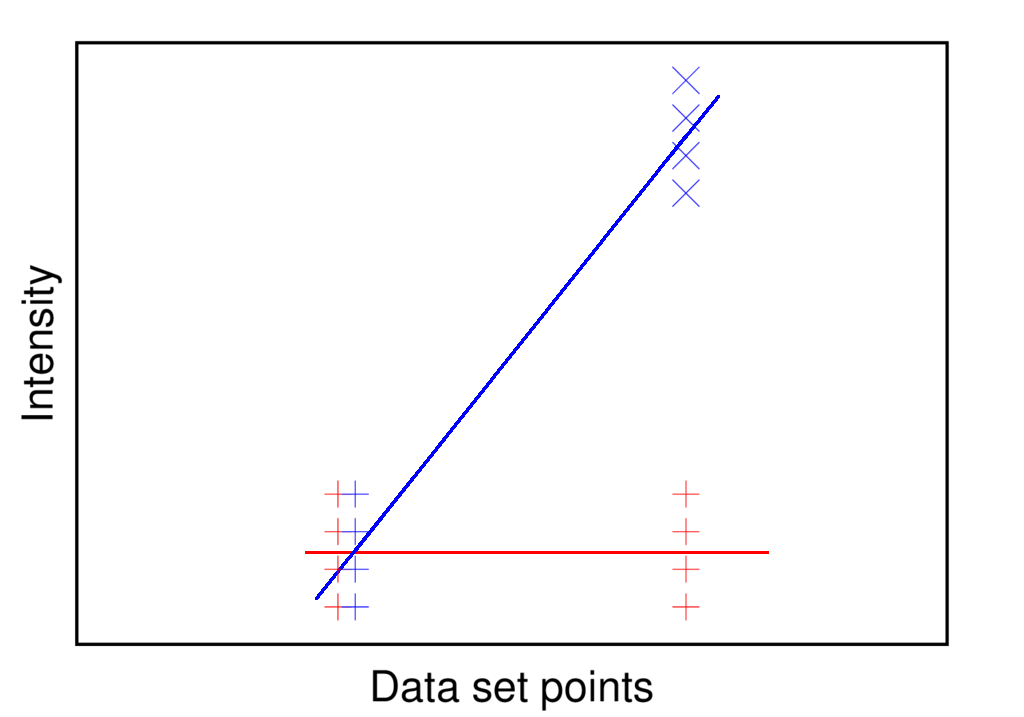
\includegraphics[width=0.7\textwidth]{./IMAGES/MOD-TARPROT/tarprot-ancova.png}	    
	\caption[Data organization prior to the ANCOVA test]{\textbf{Data organization prior to the ANCOVA test.} Two data sets with two points each are created, one data set for the control (red) and one for a given experiment (blue). The intensity data in the replicates of the control is used in both data points for the control (+) and in the first data point of the given experiment. The intensity data in the replicates of the given experiment is used for the second point of the data set for the given experiment (x). After this, the best fitting line for each data set is found and the slopes of the lines are compared in a test for homogeneity of the regression slopes.} 
	\label{fig:enzdigAncova}
	\vspace{-5pt} 	
\end{figure} 

\section{The output files}

All the output generated by the Targeted Proteolysis module will be contained in a TarProt folder created inside the selected Output folder. If the Output folder field in the section \textit{Files} in Region \num{2} of the interface is left empty, then the TarProt folder will be created in the directory containing the data file. If the selected Output folder already contains a TarProt folder, then the current date and time to the seconds will be added to the name in order to avoid overwriting files from previous analyses. By default the TarProt folder will contain four files with extensions .tarprot, .cutprop, .filtpept and uscr and a Data{\_}Steps folder. The name of these files is provided with the Output name field in the section \textit{Files} of Region \num{2} of the interface. Depending on the user provided input extra folders and files will be created inside the TarProt folder (\autoref{fig:enzdigFolder}). For the rest of this chapter we will assume that the user provided name for the Output folder was \textit{t}, the Output name was myTest, the target protein was \textit{efeB} and all optional analyses were performed.

\begin{figure}[h]
	\centering
	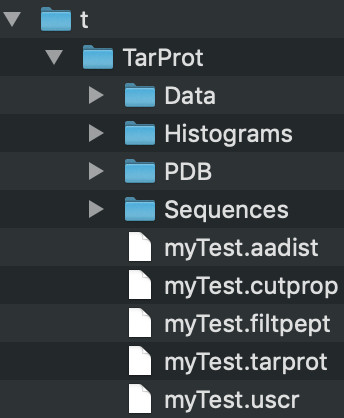
\includegraphics[width=0.35\textwidth]{./IMAGES/MOD-TARPROT/tarprot-files.jpg}	    
	\caption[The structure of the Output folder from the Targeted Proteolysis module]{\textbf{The structure of the Output folder from the Targeted Proteolysis module.} Folders Data, Histograms, PDB and Sequences are optional and will be created only if requested. The same is true for the .aadist file.} 
	\label{fig:enzdigFolder}
	\vspace{-5pt} 	
\end{figure} 

\phantomsection
If the parameter Columns to extract (see page \pageref{par:enzdigColExt}) is different than NA, then shorter versions of the data file will be created and saved in a folder Data inside the main folder t. The folder t/TarProt/Data will\label{par:datafilesenzdig} contain three files as described in \autoref{subsec:shortDF}.

If the parameter Histograms window (see page \pageref{par:enzdigHist}) is different than NA, then histograms of the detected cleavage sites will be created as described in \autoref{subsec:histocut}. The folder t/TarProt/Histograms will contain two files with the histograms.

If a PDB file was selected and the parameter PDB ID  (see page \pageref{par:pdbID}) was set, then the detected cleavage sites are mapped to the structure in the .pdb file, as described in \autoref{subsec:cut2pdb} and the resulting .pdb files are saved in the folder t/TarProt/PDB. The information regarding the cleavages is saved to the beta field of the .pdb files. The .pdb files can be visualized with VMD, PyMol or Chimera. 
  
If the parameter Sequence length (see page \pageref{par:enzdigSeqL}) is different than NA, then sequence alignment files will be created as described in \autoref{subsec:seqali}. The folder t/TarProt/Sequences will contains several sequence alignment files. These are plain text files that can be viewed with any text editor.

If the parameter Positions (see page \pageref{par:enzdigPos}) is different than NA, then an AA distribution analysis is performed as described in \autoref{subsec:aadistcalc}. The file t/TarProt/myTest.aadist contains the AA distribution analysis.

The file myTest.cutprop contains the results of the number of cleavages per residue as discussed in \autoref{subsec:cutsperres} while the file myTest.filtpept contains the list of FP as described in \autoref{subsec:filtpeptfile}. The file myTest.uscr is the input file that can be used to quickly reanalyzed the data file without having to type in all the information needed by the module, see \autoref{subsec:uscrfile} for more details. 

The main output of the Targeted Proteolysis module is the myTest.tarprot file. This file contains a summary of the user provided input and a table specifying the FP for each experiment. In addition, this file contains the information necessary to visualize the fragments generated during the experiments and to run all optional analyses individually without having to run the entire module.

\section{Visualizing the output files}

After the analysis of the Targeted Proteolysis module is finished new windows will appear showing a graphical representation of the results contained in the .tarprot and .cutprop files. Depending on the user input, the AA distribution analysis and the histogram for the cleavage sites in the recombinant protein will also be shown. More details about the graphical representation of the .aadist, .hist and .cutprop files is given in \autoref{subsec:aadistcalc}, \autoref{subsec:histocut} and \autoref{subsec:cutsperres} respectively. The data contained in the shorter versions of the input file and the sequence alignment files can be easily viewed using any text editor.   

The window displaying the results in the .tarprot file is divided in four regions (\autoref{fig:enzdigfra}).

\begin{figure}[h]
	\centering
	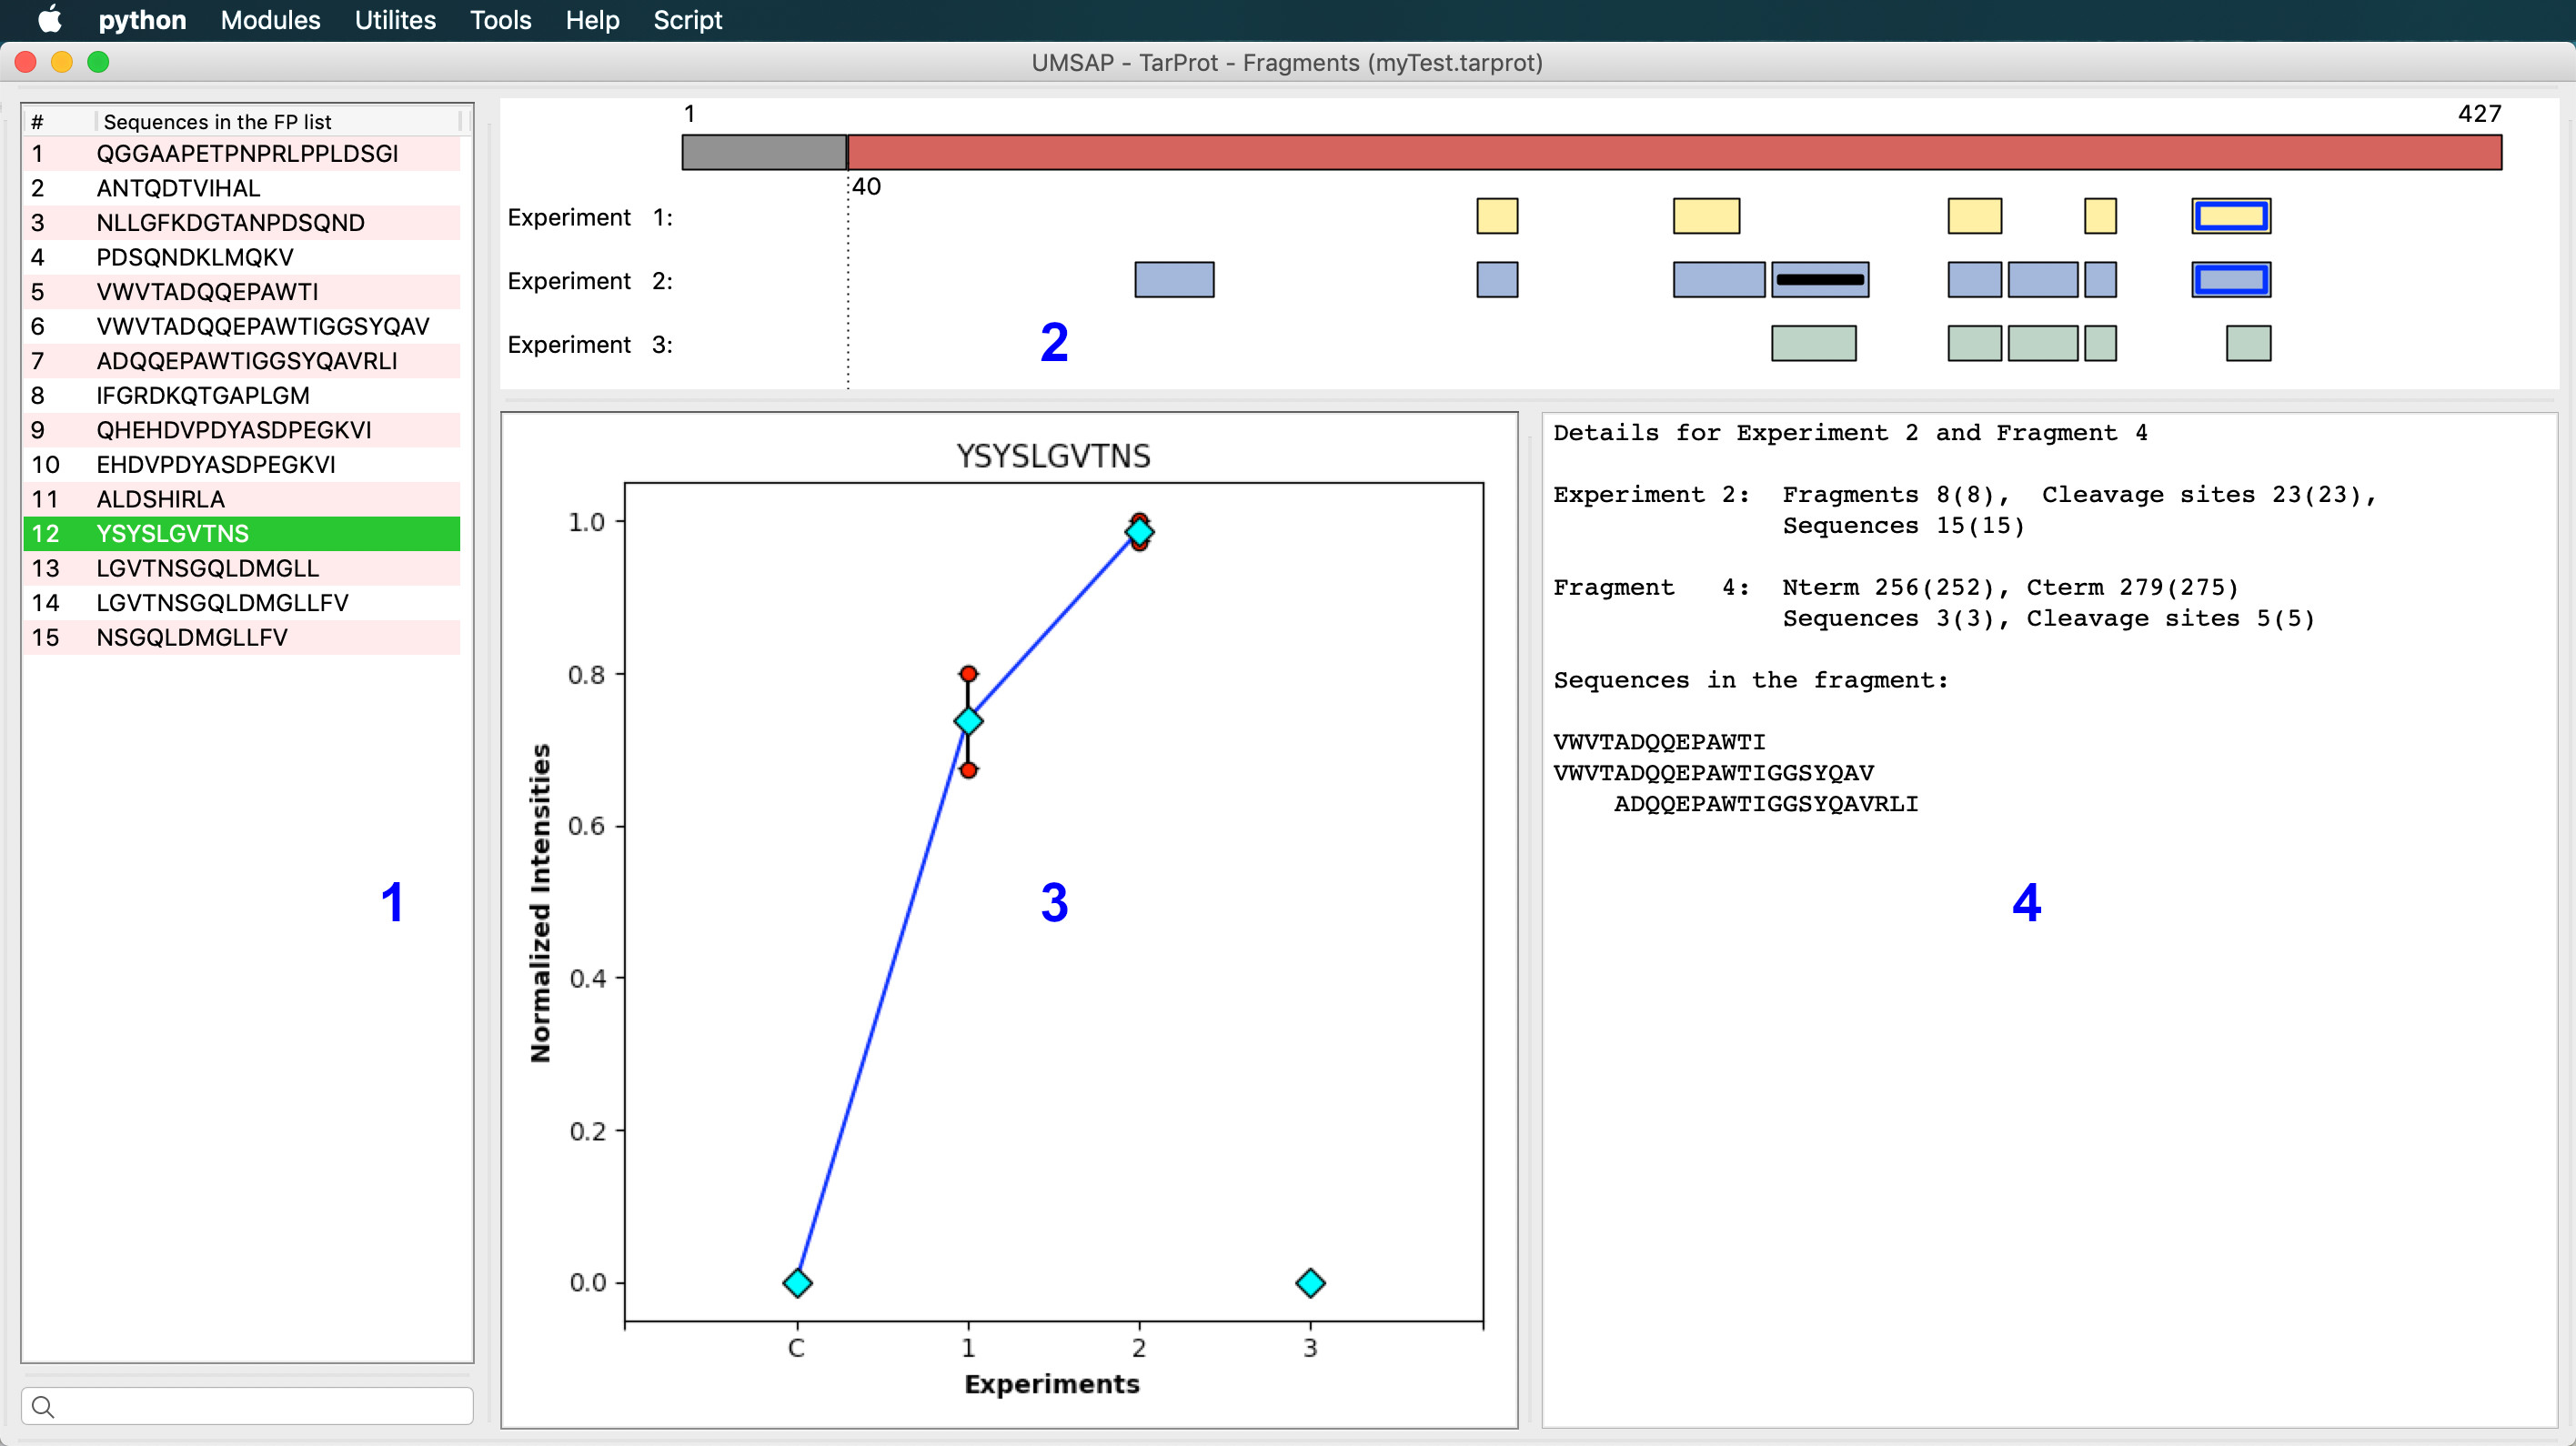
\includegraphics[width=0.8\textwidth]{./IMAGES/MOD-TARPROT/tarprot-frag.jpg}	    
	\caption[The Fragment analysis window]{\textbf{The Fragment analysis window.} Users can performed here the analysis of the fragments obtained in the enzymatic proteolysis experiments.} 
	\label{fig:enzdigfra}
	\vspace{-5pt} 	
\end{figure} 

Region \num{1} contains a list box displaying the complete list of FP. Selecting one sequence in the list box will highlight the fragments in Region \num{2} containing the selected peptide with a blue thicker border. In addition, a plot of Normalized intensities vs experiment number for the selected peptide will be displayed in Region \num{3}. Below the list box there is a search box that allows to search for a sequence in the FP list. If the typed sequence exactly matches one peptide of the FP list, then the sequence will be selected in the list box, the fragments containing the sequence in Region \num{2} will be highlighted and the plot in Region \num{3} will be updated. If the typed sequence is found in more than one peptide of the FP list, the number and the sequence of the peptides containing the typed sequence will be shown.

Region \num{2} displays all the fragments generated in the enzymatic proteolysis experiment. The first line represent the full sequence of the recombinant protein. The red color represents residues from the native protein while the gray color represents residues in the recombinant protein that do not belong to the native protein sequence. The other rows represent the different experiments performed. The experiments are organized in the same way as specified with the parameter Results - Control experiments in Region \num{2} of the interface of the Targeted Proteolysis module, see page \pageref{par:results}. In addition, vertical dotted lines are drawn from the recombinant protein sequence to the bottom of Region \num{2} in order for users to quickly identified if fragments contain only residues from the native protein or not. Selecting one fragment will highlight the fragment with a black line and will give detailed information about the fragment in Region \num{4}. 

Region \num{3} will display a plot of Normalized intensities vs experiment number. The plot will display the data for a single FP selected in the list box in Region \num{1}. The values in the plot are obtained by using feature rescaling to bring all intensity values for the selected peptide into the range \numrange{0}{1}. Discarded replicates are not shown and if intensity values were normalized prior to the Targeted Proteolysis analysis then the normalized values are used for the feature rescaling procedure. The values for replicates are shown as red circles. The average for a given experiment is shown as bigger cyan diamonds and the standard deviation is used for the bars. The blue lines only connect the control experiment and experiments showing intensity values significantly different at the chosen significance level.  

Region \num{4} will display detailed information about a selected fragment in Region \num{2}. In this Region regular numbers refer to the recombinant protein sequence while number between parenthesis refers to the Native sequence. The Experiment section in the text contain information about the experiment in which the fragment was identified. The information includes the total number of fragments, the total number of sequences and the total number of unique cleavage sites identified in the experiment. The Fragment section in the text gives similar information about the selected fragment and also includes the first and last residue numbers in the fragment. The rest of the lines show a sequence alignment of all the peptides in the fragment.

\subsection{The Tools menu}

The Tools menu in the window allows to extend the functionality of the windows. Through this menu users can create a copy of the FP list, save an image of the fragments or the plot and reset the state of the window. Most of these functions can be also accessed by clicking the right button of the mouse (\autoref{fig:enzdigfra}).